\documentclass[aspectratio=1610,xcolor=dvipsnames]{beamer}
\usepackage{theme}
\usepackage[utf8x]{inputenc}

\usepackage[english]{babel}
\usepackage{calligra}
\usepackage{subcaption}
\usepackage{hyperref}

% Graphics and video
\usepackage{graphicx,float,wrapfig}
\usepackage{animate}
% \usepackage{media9}
% \usepackage{multimedia}
\graphicspath{
  {../assets/}%
}
% \addmediapath{
%     ../assets/
% }

\renewcommand{\bold}[1]{\textbf{\structure{#1}}}

  
\author[Conti \and Daniotti]{Samuele Conti \and Filippo Daniotti}
\title[Global Motion Estimation]{\textsc{Global Motion Estimation}}
\subtitle{A robust and hierarchical approach}
\institute[DISI - University of Trento]{Department of Information Engineering\\and Computer Science}
\date{April 20, 2022}


\AtBeginSection[]
{
    \begin{frame}
        \frametitle{Table of Contents}
        \tableofcontents[currentsection]
    \end{frame}
}

\begin{document}

\begin{frame}
    \titlepage
    \begin{figure}[H]
        \begin{center}
            
\includegraphics[width=0.4\linewidth]{marchio_unitrento_colore_it_202002.eps}
        \end{center}
    \end{figure}
\end{frame}

\begin{frame}
    \tableofcontents[sectionstyle=show,subsectionstyle=show/shaded/hide,subsubsectionstyle=show/shaded/hide]
\end{frame}

\section{Introduction}
\begin{frame}{Introduction}
    In this work we are going to present:
    \begin{itemize}
        \item a broad introduction to the problem of global motion estimation
        \item an overview of the theoretical foundations of our solution
        \item the framework we developed from the aforementioned literature
        \item an analysis of the performances of our solution
        \item a brief discussion of the limitations and possible improvements
    \end{itemize}
\end{frame}

\section{The problem}
\begin{frame}{Motion estimation}
    The problem of motion estimation aims to produce an estimate of the movement of the objects in a video
    \bigskip
    \begin{itemize}
        \item idea: the difference between two frames gives information on the motion in the scene
        \item ideally, we could be able to estimate the direction and velocity of any object of interest
        \item in fact, the problem is quite convoluted
        \begin{columns}
            \begin{column}{0.4\textwidth}
                \begin{itemize}
                    \item the motion in a scene is often a combination of multiple moving object
                    \item alongside local motion of actors, there may be camera movements that affect the whole image
                \end{itemize}
            \end{column}
            \begin{column}{0.4\textwidth}
                \begin{center}
                    \animategraphics[loop,autoplay,width=.7\linewidth]{20}{gifs/pan240/pan240-}{0}{40}
                \end{center}
            \end{column}
        \end{columns} 
    \end{itemize}
\end{frame}

\begin{frame}{Global motion stimation}
    Global motion estimation aims to compute an estimate of the global motion patterns introduced by the camera
    \bigskip
    \begin{itemize}
        \item \textit{camera movements described motion models projectve polynomial affine}
        \item removing camera motion is useful in a virety of applications:
        \begin{itemize}
            \item when dealing unwanted motion from a video 
            \item when we are interested in the ego-motion
        \end{itemize}
    \end{itemize}    
\end{frame}

\section{Literature}
\begin{frame}{Dealing with GME}
    Most of the existing algorithms that deal with global motion estimation assume that camera motion can be described as a  \bold{parameterized motion model}.
    \begin{block}{Parameterized motion model}
        It is an equation that describes the expected shape of the motion vector for each still pixel, given a certain movement of the camera
    \end{block}
    \bigskip
    Different models describe different types of motion (translation, rotation, panning, et cetera)
    \begin{exampleblock}{Well-established models}
        \begin{itemize}
            \item translation model
            \item affine model (our choice)
            \item projective model
        \end{itemize}
    \end{exampleblock}
\end{frame}

\begin{frame}{Estimating parameters}
    Once the choice of the motion model has been made, there are two main approaches for estimating the parameters
    \bigskip
    \begin{itemize}
        \item direct methods
        \item indirect methods
    \end{itemize}
    \bigskip
    For our solution we went for \bold{indirect} methods
\end{frame}

\section{Implementation}
\begin{frame}{Overview}
    Three are the main operations that constitute the framework that we have developed:
    \bigskip
    \begin{enumerate}
        \item \bold{motion estimation}: compute a dense motion field for a given frame
        \item \bold{global motion estimation}: compute the motion model parameters
        \item \bold{motion compensation}: subtract GME from the dense motion field to get a compensated frame
    \end{enumerate}
\end{frame}

\subsection{Dense motion estimation}
\begin{frame}{Block-based motion estimation}
	The affine model requires a dense motion field when computing the parameters, which we compute via a block-based approach

	\bigskip	
	We started with 3 well-established BBME algorithms:
	\begin{itemize}
		\item exhaustive search
		\item three-step search
		\item 2D log search
	\end{itemize}
    Then, we search for new algorithms in the literature and landed on \bold{diamond search}
	\bigskip
    \begin{block}{Displaced frame difference}
        As DFD, we tried both 1-norm (MAE) and 2-norm (MSE)        
    \end{block}
    
\end{frame}

\begin{frame}{Exhaustive search}
	\begin{figure}
		\begin{minipage}{.45\textwidth}
            \centering
            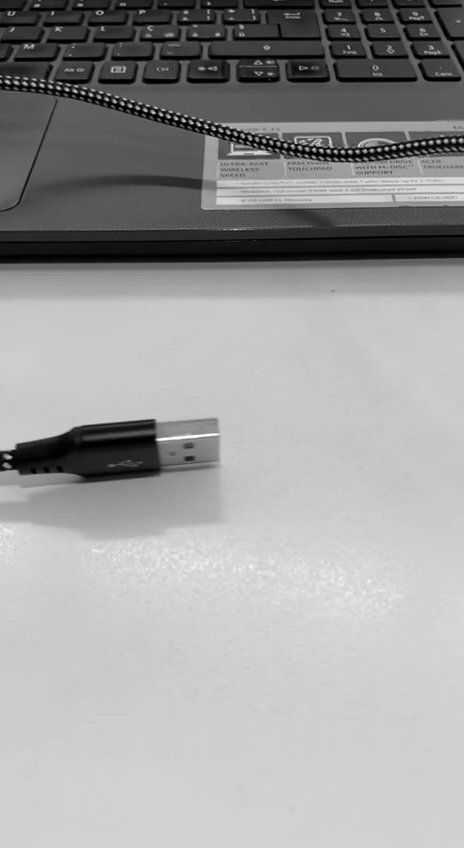
\includegraphics[keepaspectratio, width=.55\linewidth]{images/bbme-im.png}
            \subcaption{Target frame}
            \label{fig:bbme-0-im}
		\end{minipage}
		\begin{minipage}{.45\textwidth}
            \centering
            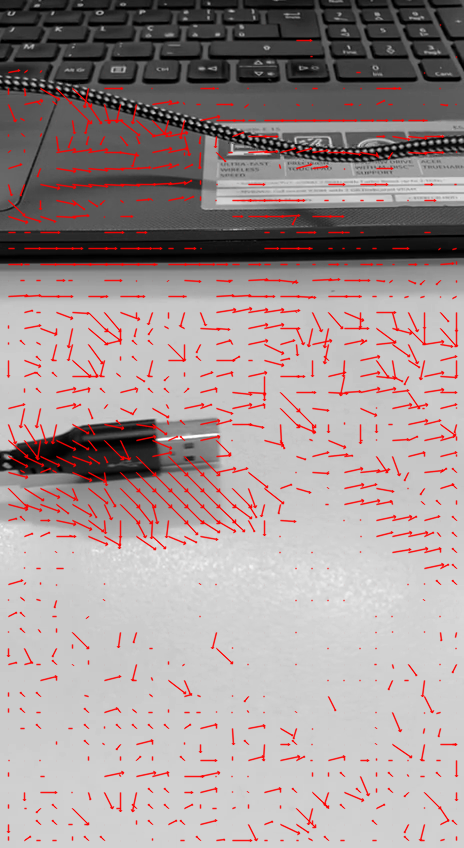
\includegraphics[keepaspectratio, width=.55\linewidth]{images/bbme-0-res.png}
            \subcaption{Needle diagram}
            \label{fig:bbme-0-res}
		\end{minipage}
        \label{fig:bbme-0}
        \caption{Motion field result of our EBBME implementation}
	\end{figure}
\end{frame}

\begin{frame}{Three-step search}
	\begin{figure}[H]
		\begin{minipage}{.45\textwidth}
            \centering
            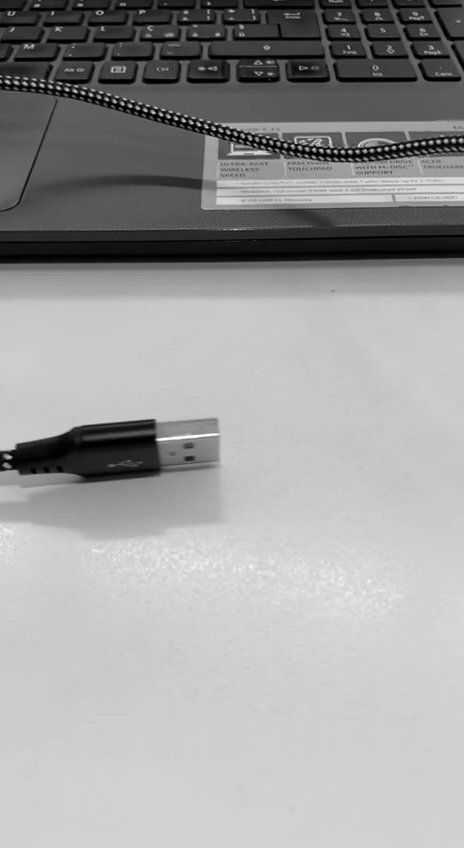
\includegraphics[keepaspectratio, width=.55\linewidth]{images/bbme-im.png}
            \subcaption{Target frame}
            \label{fig:bbme-1-im}
		\end{minipage}
		\begin{minipage}{.45\textwidth}
            \centering
            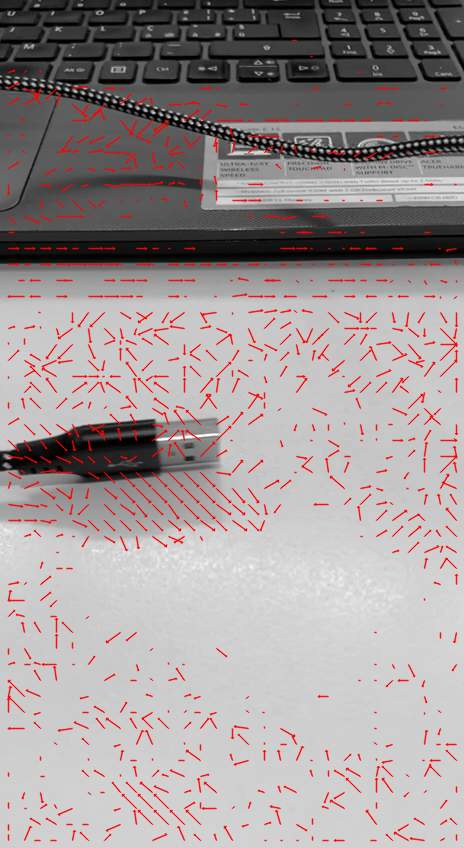
\includegraphics[keepaspectratio, width=.55\linewidth]{images/bbme-1-res.png}
            \subcaption{Needle diagram}
            \label{fig:bbme-1-res}
		\end{minipage}
        \label{fig:bbme-1}
        \caption{Motion field result of our TSS implementation}
	\end{figure}
\end{frame}

\begin{frame}{Hierarchical TSS}
    \begin{figure}[H]
		\begin{minipage}{.45\textwidth}
            \centering
            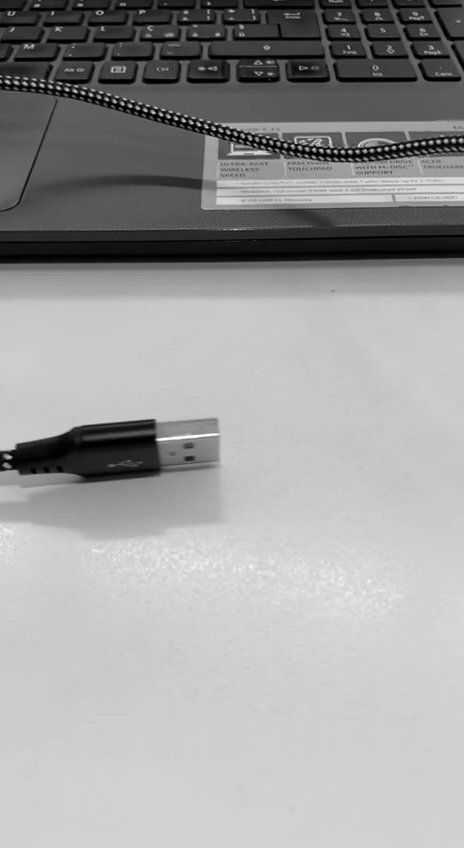
\includegraphics[keepaspectratio, width=.55\linewidth]{images/bbme-im.png}
            \subcaption{Target frame}
            \label{fig:bbme-1-im}
		\end{minipage}
		\begin{minipage}{.45\textwidth}
            \centering
            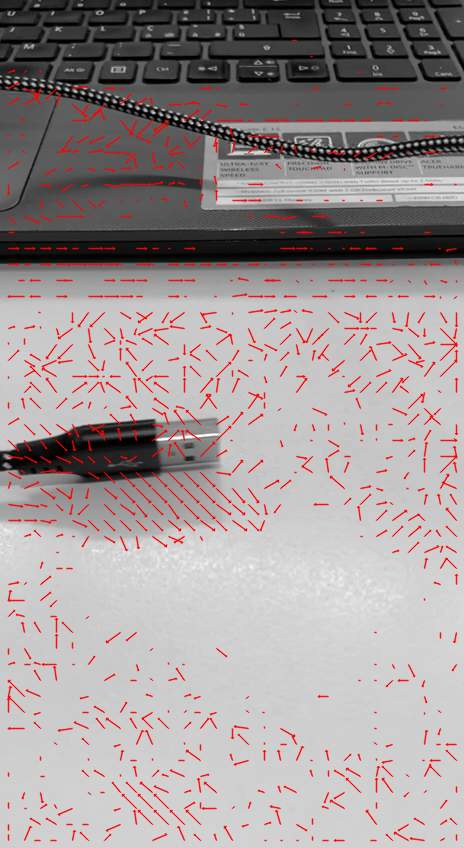
\includegraphics[keepaspectratio, width=.55\linewidth]{images/bbme-1-res.png}
            \subcaption{Needle diagram}
            \label{fig:bbme-1-res}
		\end{minipage}
        \label{fig:bbme-1}
        \caption{Motion field result of our TSS implementation}
	\end{figure}
\end{frame}

\begin{frame}{2D Log search}
	\begin{figure}
		\begin{minipage}{.45\textwidth}
            \centering
            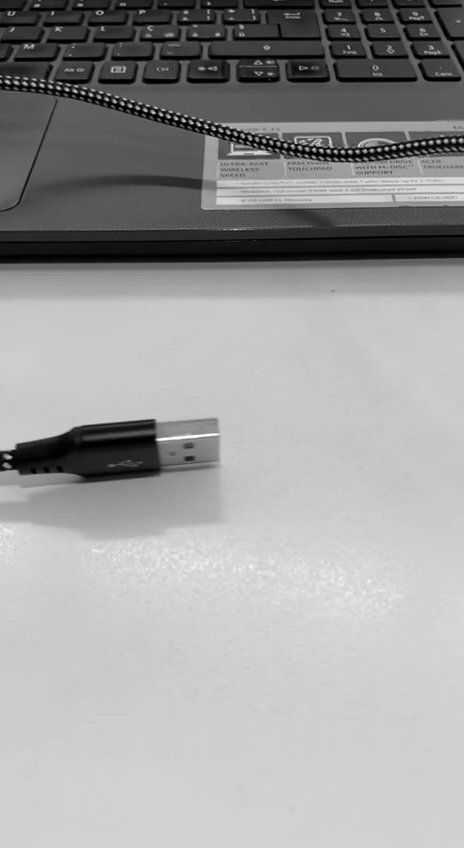
\includegraphics[keepaspectratio, width=.55\linewidth]{images/bbme-im.png}
            \subcaption{Target frame}
            \label{fig:bbme-2-im}
		\end{minipage}
		\begin{minipage}{.45\textwidth}
            \centering
            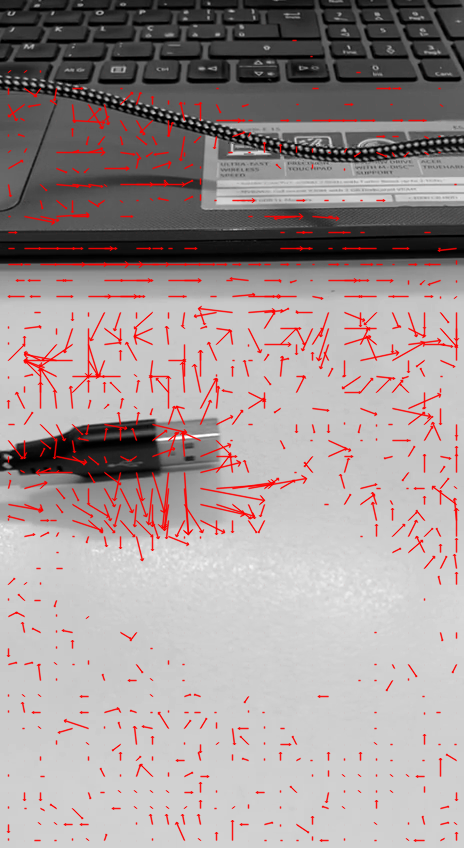
\includegraphics[keepaspectratio, width=.55\linewidth]{images/bbme-2-res.png}
            \subcaption{Needle diagram}
            \label{fig:bbme-2-res}
		\end{minipage}
        \label{fig:bbme-2}
        \caption{Motion field result of our TDLS implementation}
	\end{figure}
\end{frame}

\subsubsection*{Diamond search BBME}
\begin{frame}{Diamond search}
	BBME algorithm presented in Zhu and Ma, 2000. Better performances thant classic algorithms (TSS) and comparable to latest (NTSS), yet more efficient in computation.

    \bigskip
    It uses two different search patterns, both of which are diamond-shaped:
    \begin{itemize}
        \item large diamond search pattern (LDSP)
        \item small diamond search pattern (SDSP)
    \end{itemize}
    \begin{figure}
        \centering
        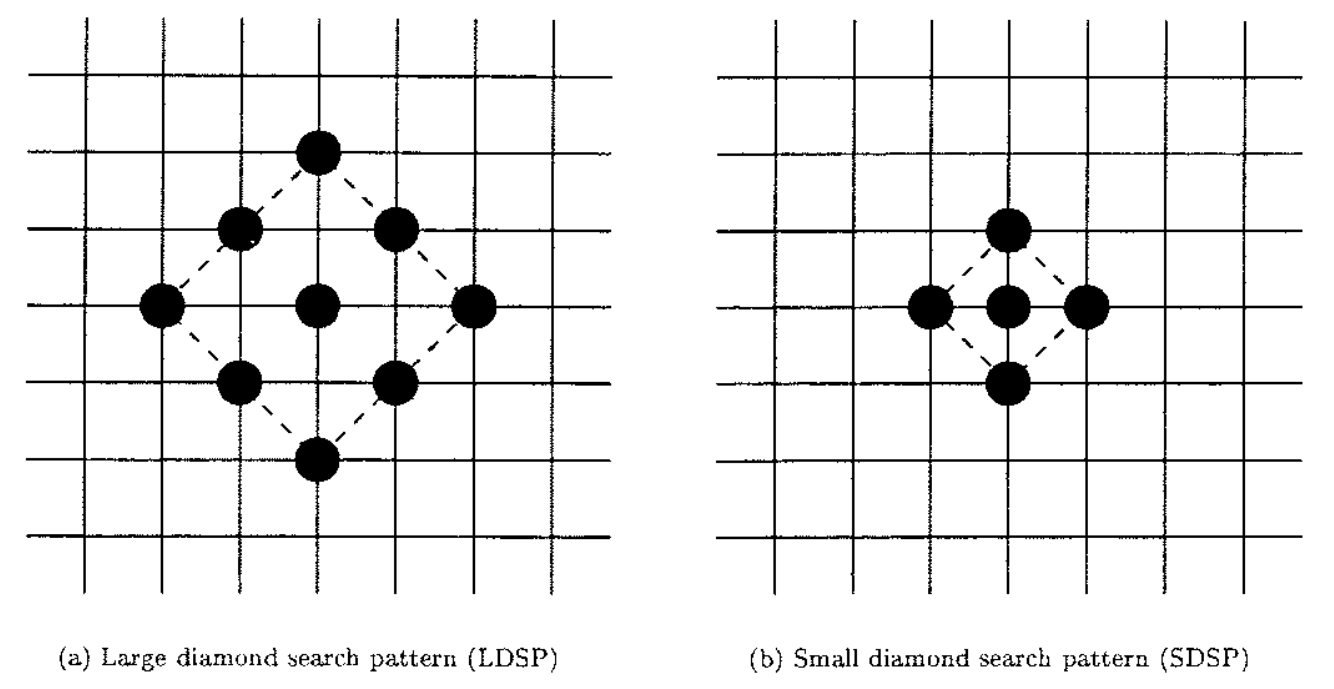
\includegraphics[keepaspectratio,width=.5\linewidth]{images/ds-search-patterns.png}
        \caption{The shape of LDSP and SDSP}
    \end{figure}
\end{frame}

\begin{frame}{DS algorithm}
    \begin{block}{Diamond search procedure}
        For each block:
        \begin{enumerate}
            \item place LDSP in the center of the block and compute DFD for every of the 9 displacement;
            \begin{itemize}
                \item if the minimum DFD is in the center position, then go to 3
                \item else, go to 2
            \end{itemize}
            \item reposition LDSP in the minimum DFD of the previous operation and recompute DFD;
            \begin{itemize}
                \item if the minimum DFD is in the center position, then go to 3
                \item else, repeat 
            \end{itemize}
            \item place SDSP, compute DFD and return coordinates of the minum DFD block as motion vector
        \end{enumerate}
    \end{block}
\end{frame}

\begin{frame}{DS algorithm visualized}
    \begin{figure}
        \centering
        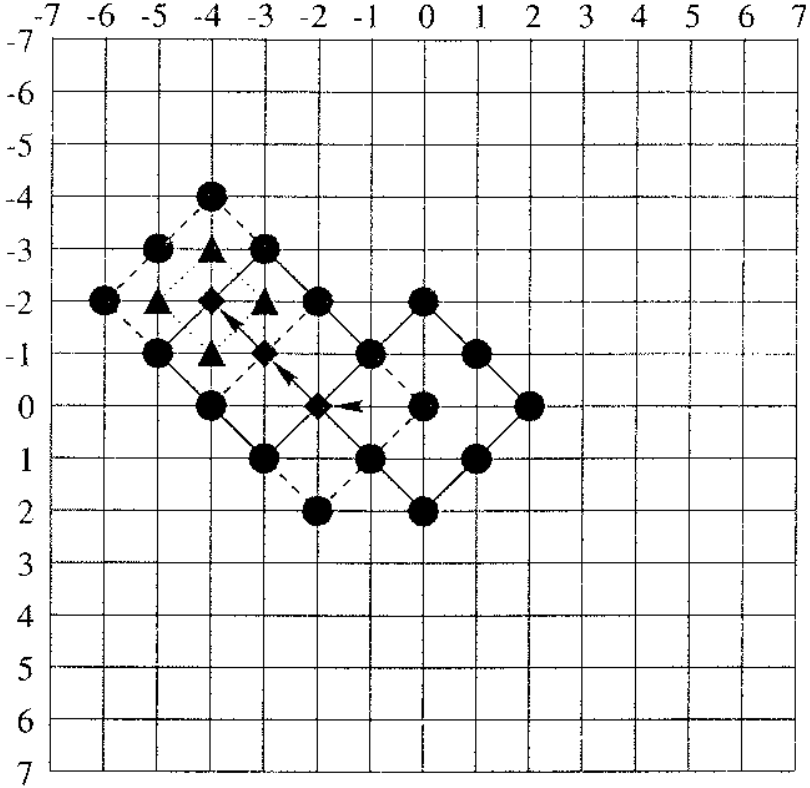
\includegraphics[keepaspectratio,width=.45\linewidth]{images/ds-exe.png}
        \caption{Example of a full execution cycle of diamond search}
    \end{figure}    
\end{frame}

\begin{frame}{DS results}
	\begin{figure}[H]
		\begin{minipage}[b]{0.45\textwidth}
            \centering
            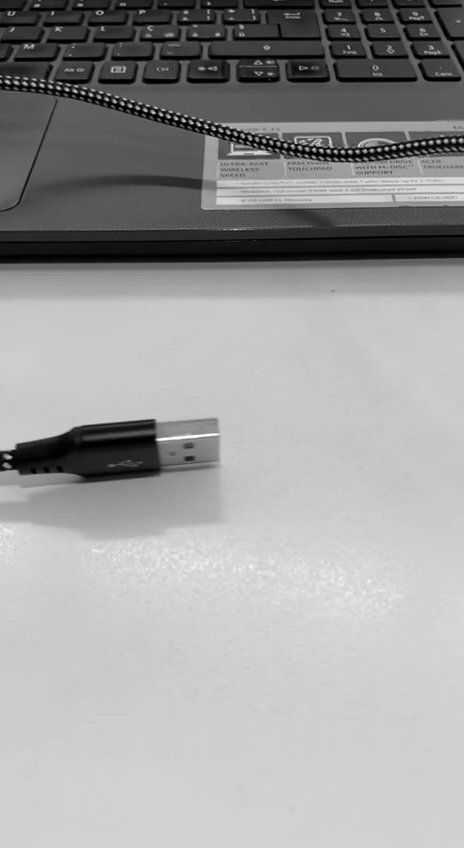
\includegraphics[keepaspectratio, width=.55\linewidth]{images/bbme-im.png}
            \label{fig:bbme-3-im}
            \subcaption{Target frame}
		\end{minipage}%
		\begin{minipage}[b]{0.45\textwidth}
            \centering
            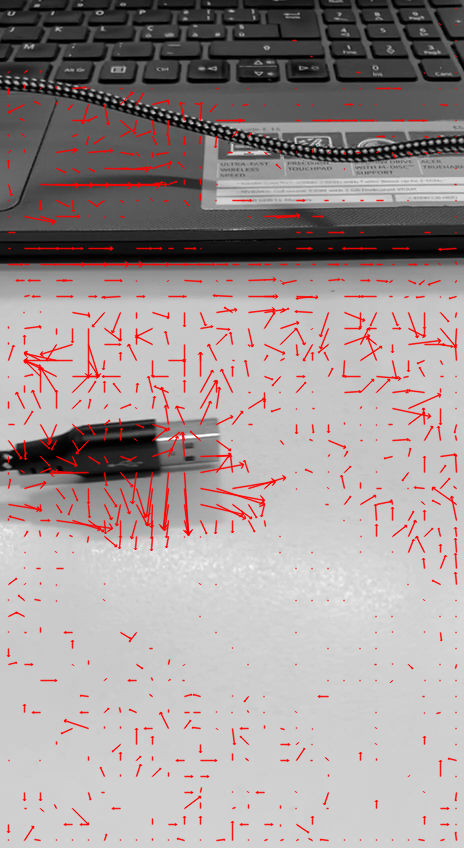
\includegraphics[keepaspectratio, width=.55\linewidth]{images/bbme-3-res.png}
            \label{fig:bbme-3-res}
            \subcaption{Needle diagram}
		\end{minipage}
        \label{fig:bbme-3}
        \caption{Motion field result of our DS implementation}
	\end{figure}
\end{frame}

\subsection{The affine model}
\begin{frame}{Affine model}
    
\end{frame}

\subsection{Refinement: robust and hierarchical GME}

\subsection{Motion compensation}
\begin{frame}{Compensation}
%     \includemedia[
%     activate=onclick,
%     width=0.5\textwidth
% ]{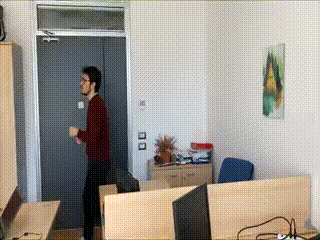
\includegraphics{gifs/pan240/pan240-0.png}}{videos/pan240.flv}
% \movie[externalviewer]{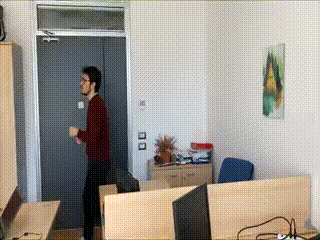
\includegraphics{gifs/pan240/pan240-0.png}}{../assets/videos/pan240.mp4}
% \href{run:../assets/videos/pan240.mp4}{text}
\end{frame}

\section{Evaluation}
\subsection{Qualitative: compensation}
\subsection{Quantitative: PSNR}

\section{Conclusions}

\begin{frame}
    \begin{center}
        {\Huge\calligra Thanks!}
    \end{center}
\end{frame}

\end{document}